% -----------------------------------------------------------------------
% Image helper functions

\newcommand{\newImage}[1]{
    \ifIMAGES
        \centering
        \IfFileExists{#1}{\includegraphics{#1}}{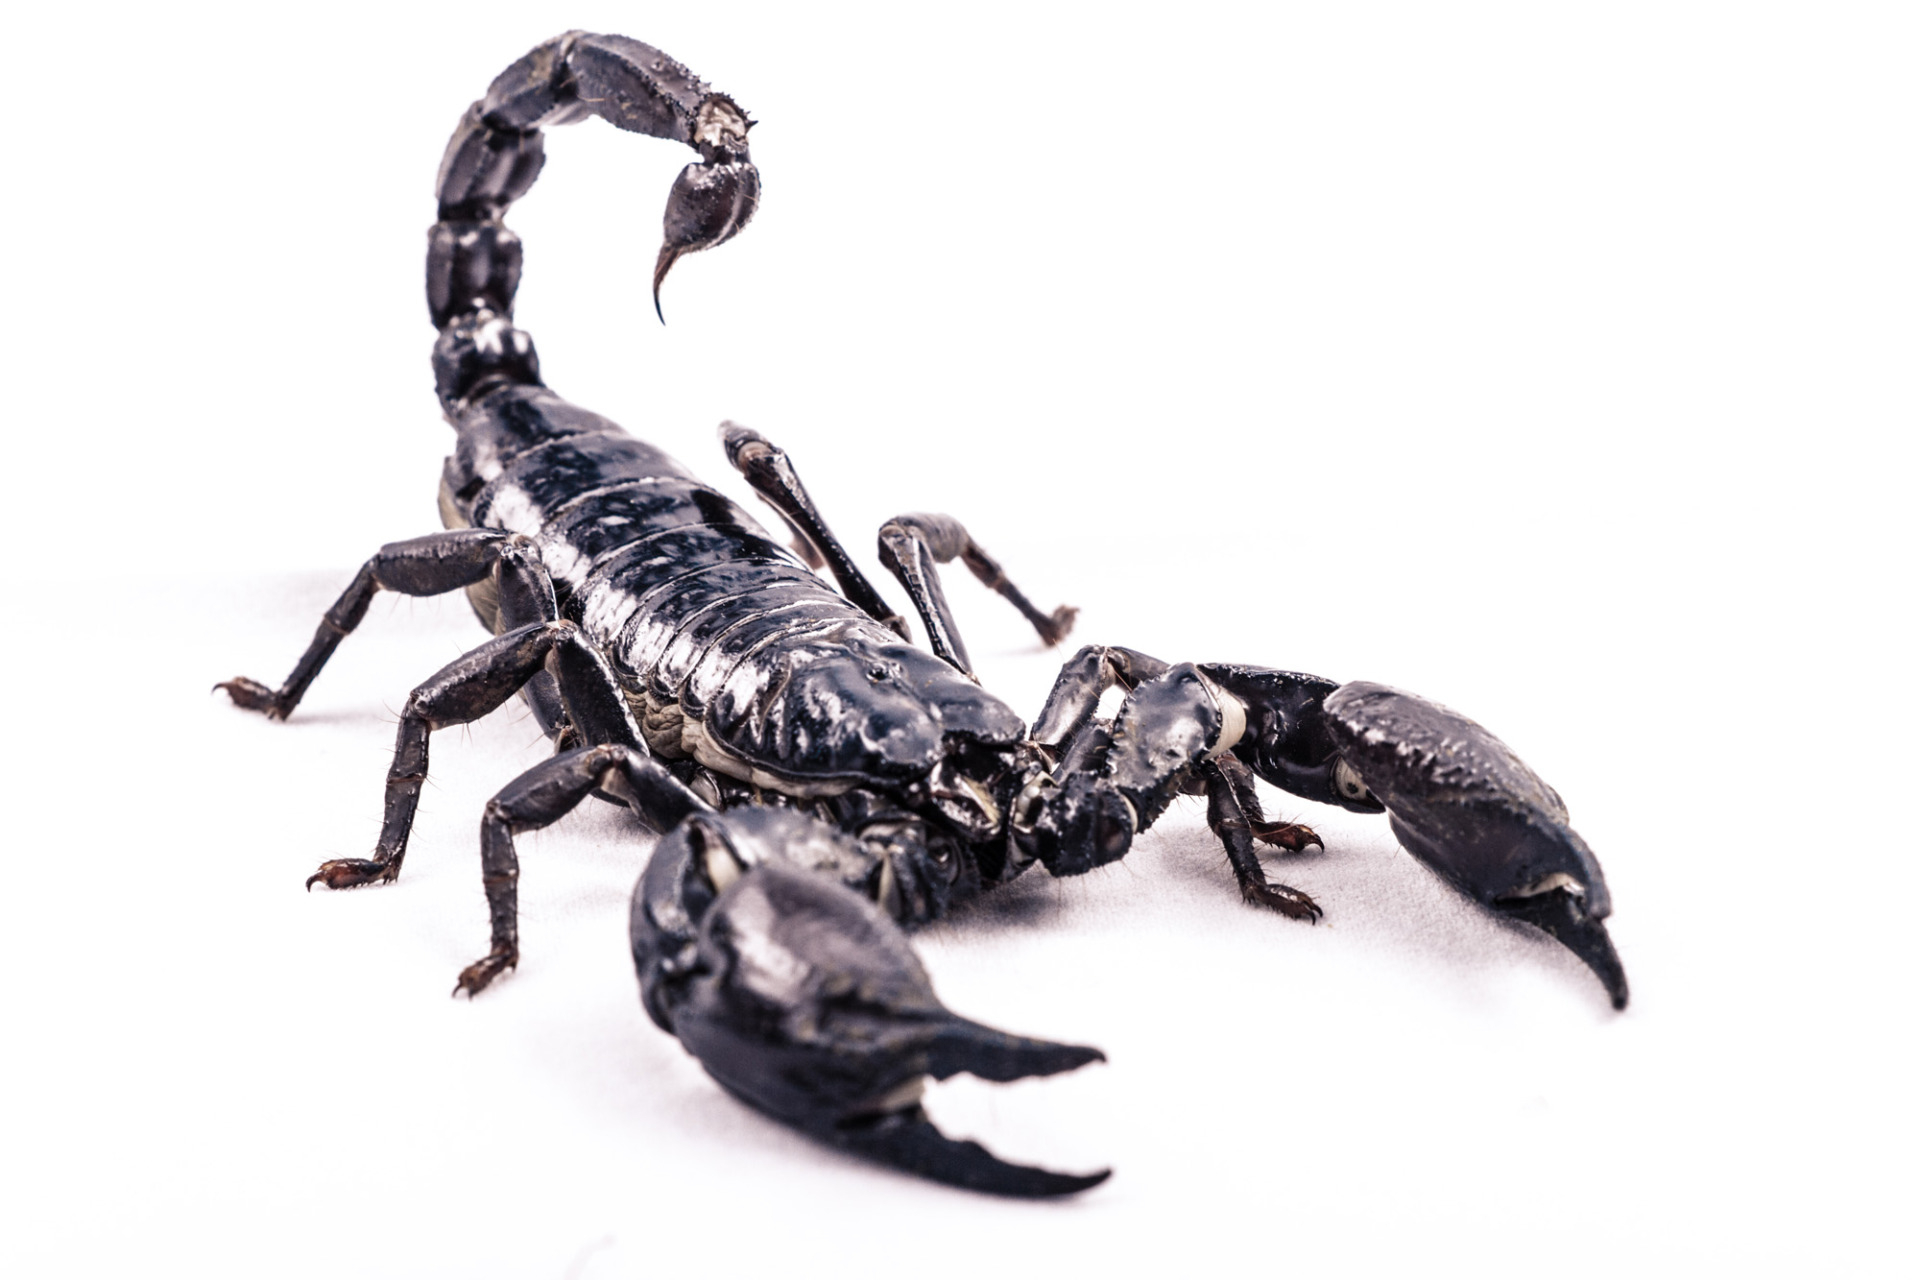
\includegraphics{figures/general/scorpion.jpg}}
    \else
    \fi
}
\newcommand{\newImageResize}[1]{
    \ifIMAGES
        \centering
        \IfFileExists{#1}{
            \resizebox{\textwidth}{!}{
                \includegraphics{#1}
            }
        }
        {
            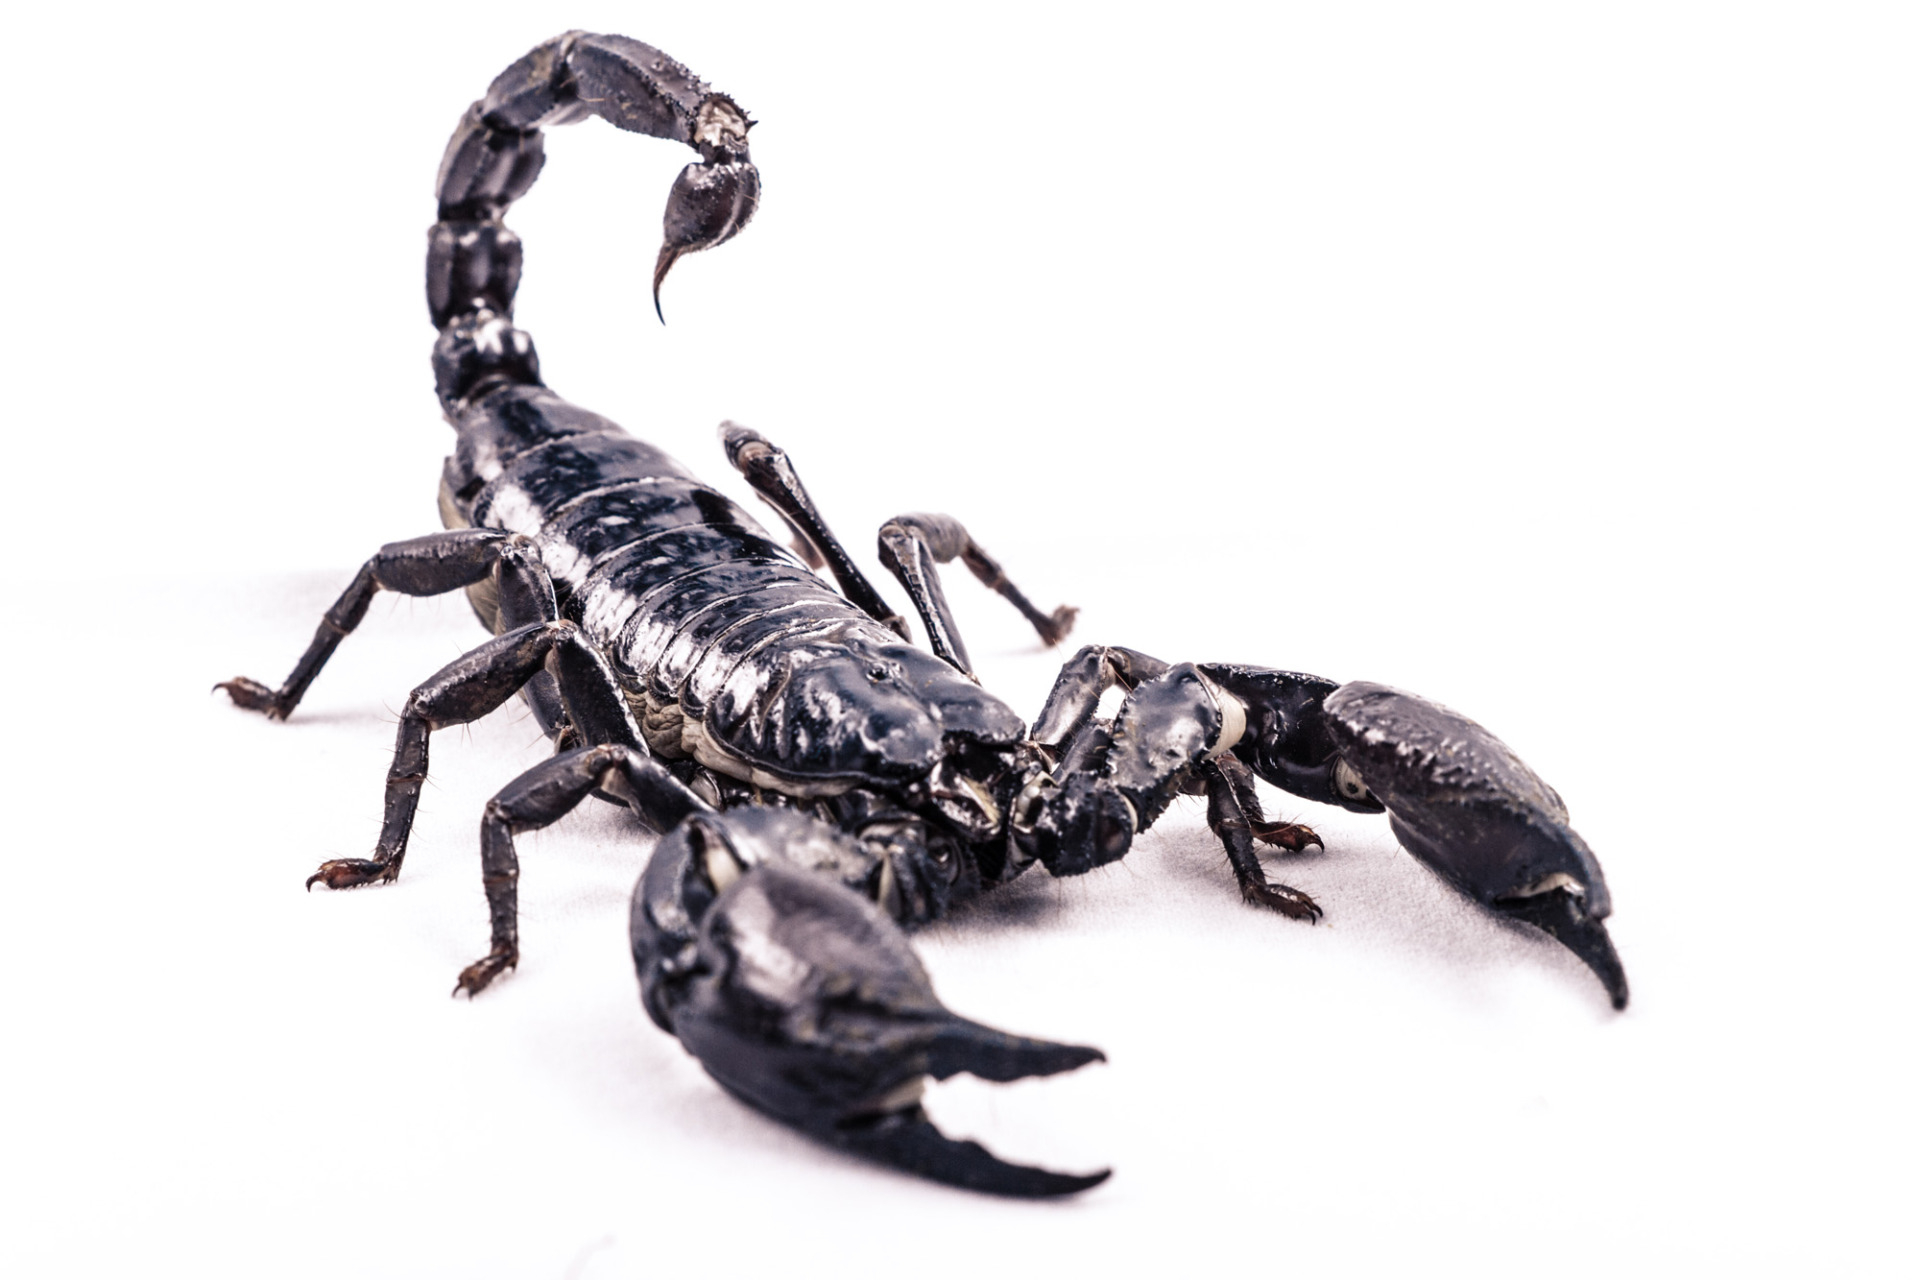
\includegraphics{figures/general/scorpion.jpg}
        }
    \else
    \fi
}
\newcommand{\newImageResizeCustom}[2]{
    \ifIMAGES
        \centering
        \IfFileExists{#2}{
            \resizebox{#1\textwidth}{!}{
                \includegraphics{#2}
            }
        }
        {
            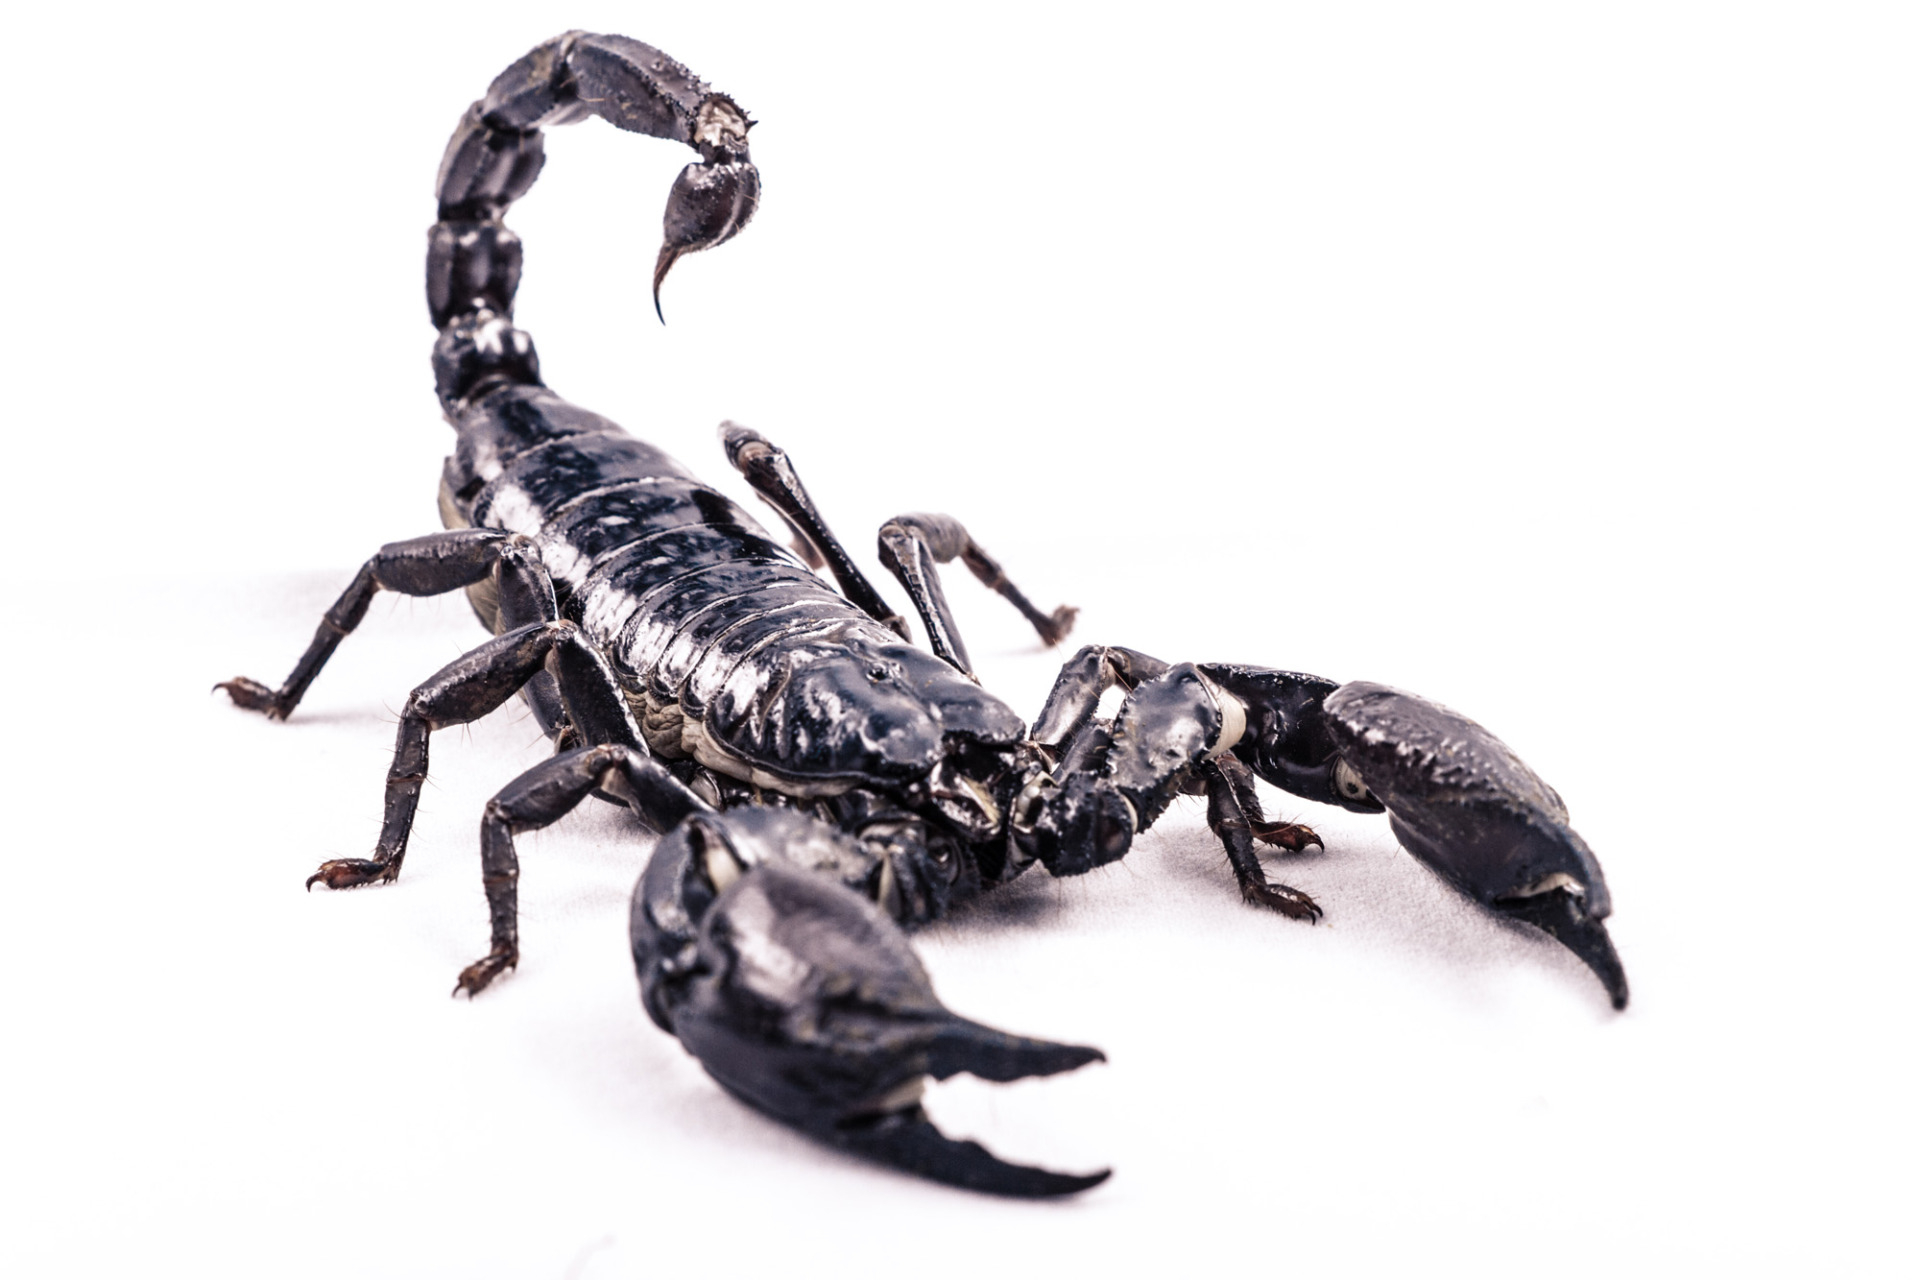
\includegraphics{figures/general/scorpion.jpg}
        }
    \else
    \fi
}
\newcommand{\newImageResizeHalf}[1]{
    \ifIMAGES
        \centering
        \IfFileExists{#1}{
            \resizebox{0.48\textwidth}{!}{
                \includegraphics{#1}
            }
        }
        {
            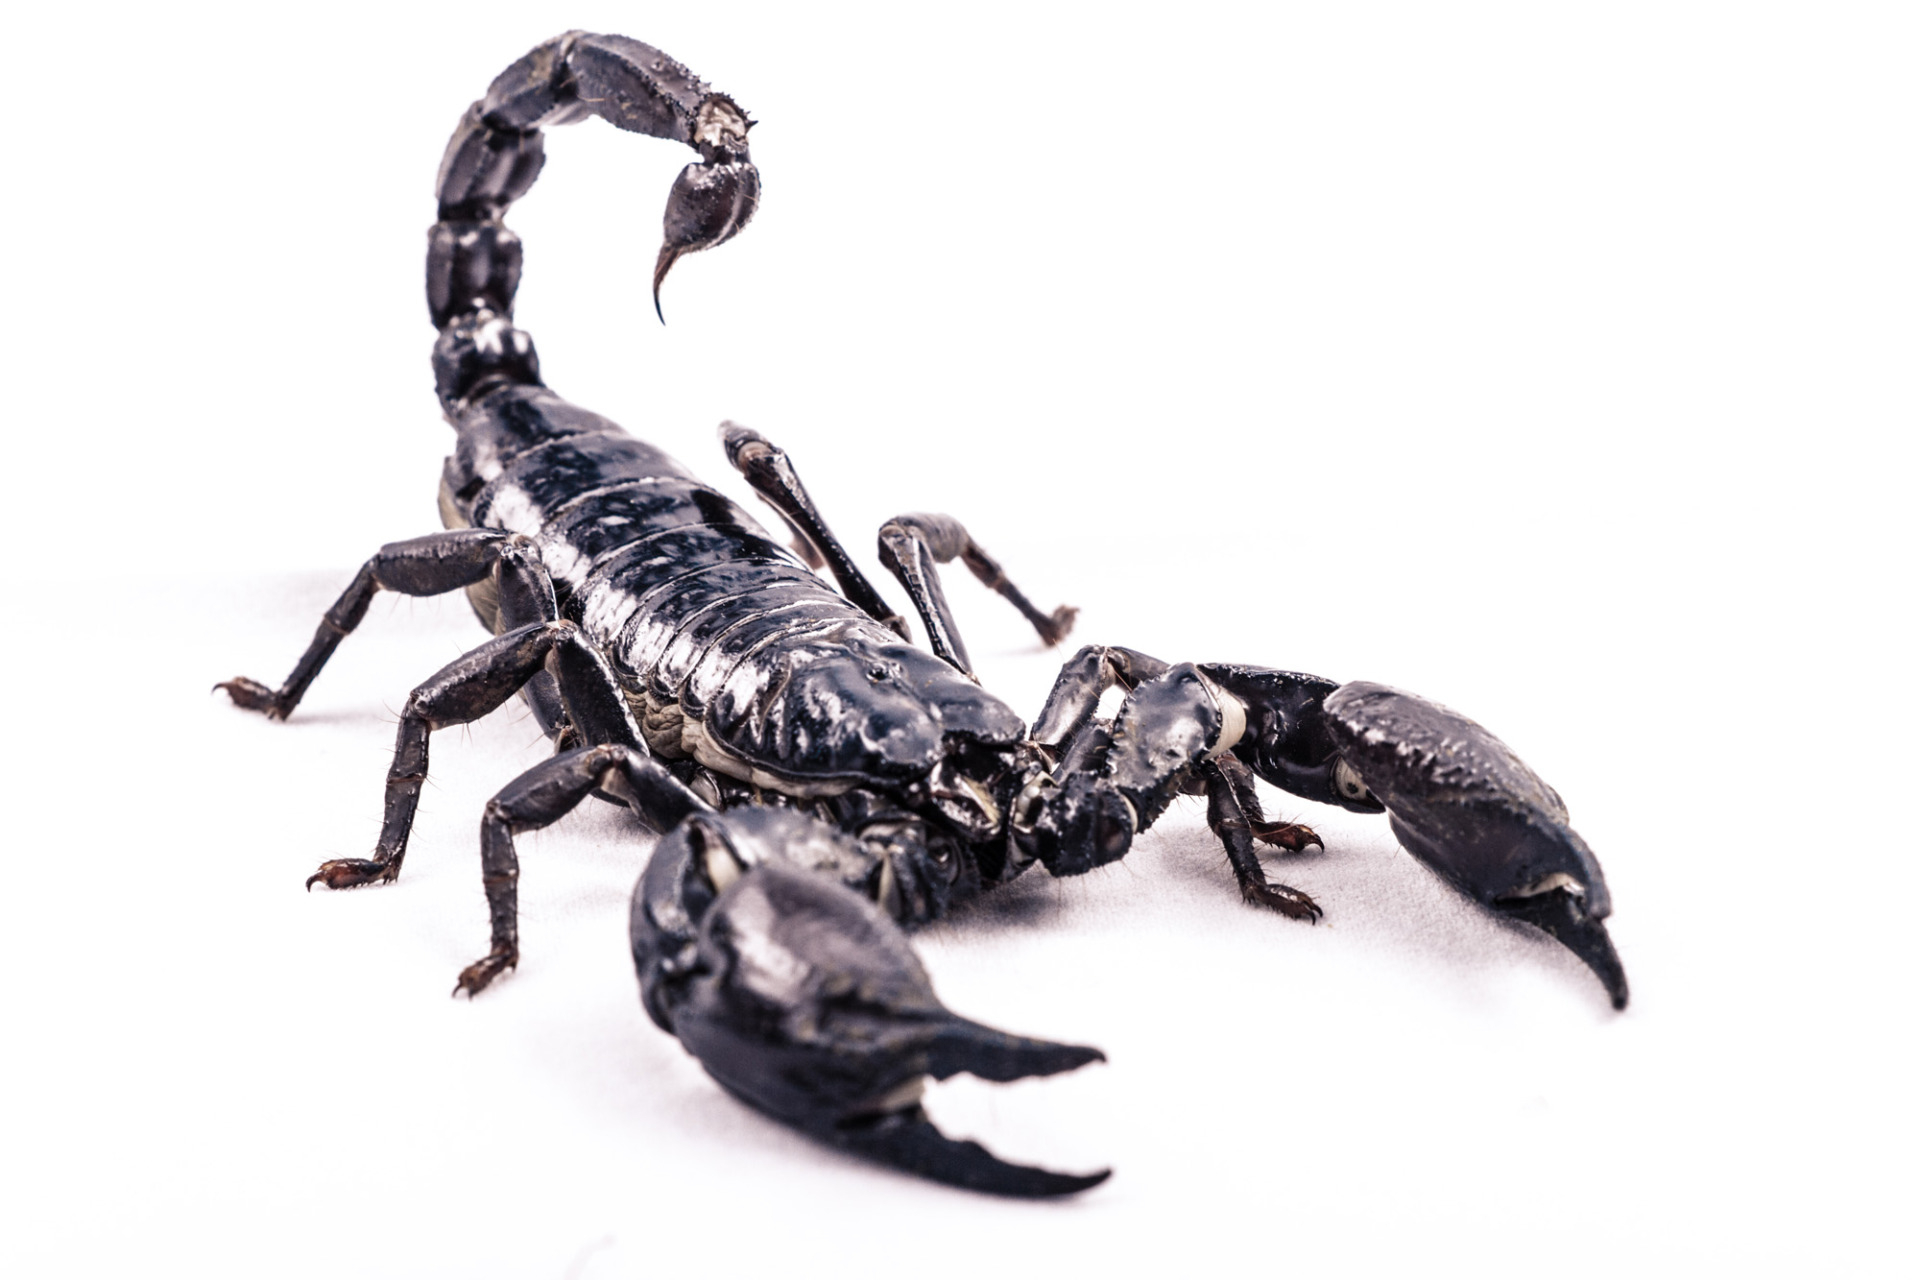
\includegraphics{figures/general/scorpion.jpg}
        }
    \else
    \fi
}
\newcommand{\newImageScale}[2]{
    \ifIMAGES
        \centering
        \IfFileExists{#1}{\includegraphics[scale=#2]{#1}}{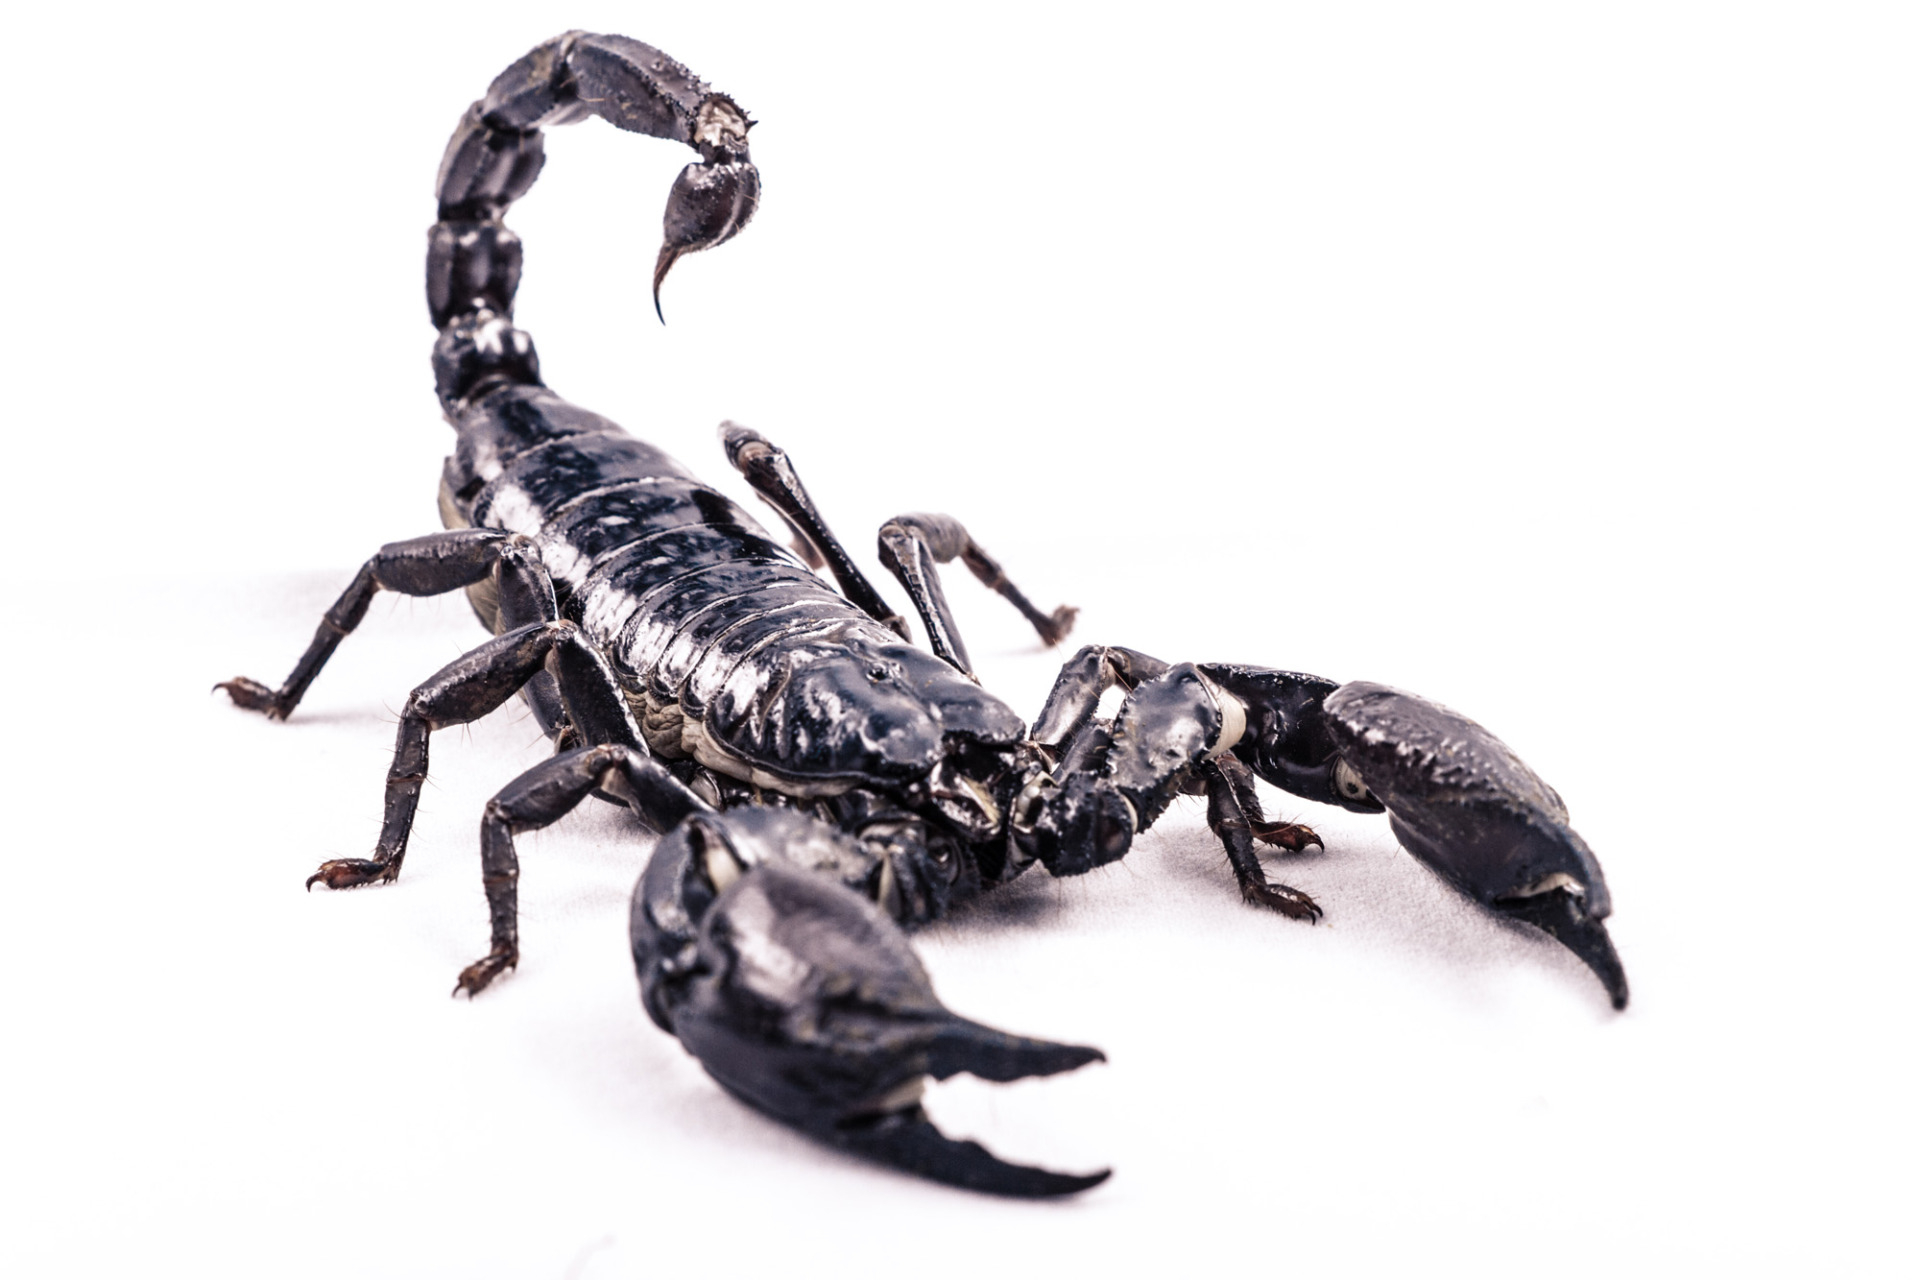
\includegraphics{figures/general/scorpion.jpg}}
    \else
    \fi
}
\newcommand{\newImageScaleRot}[2]{
    \ifIMAGES
        \centering
        \IfFileExists{#1}{\includegraphics[scale=#2,angle=-90]{#1}}{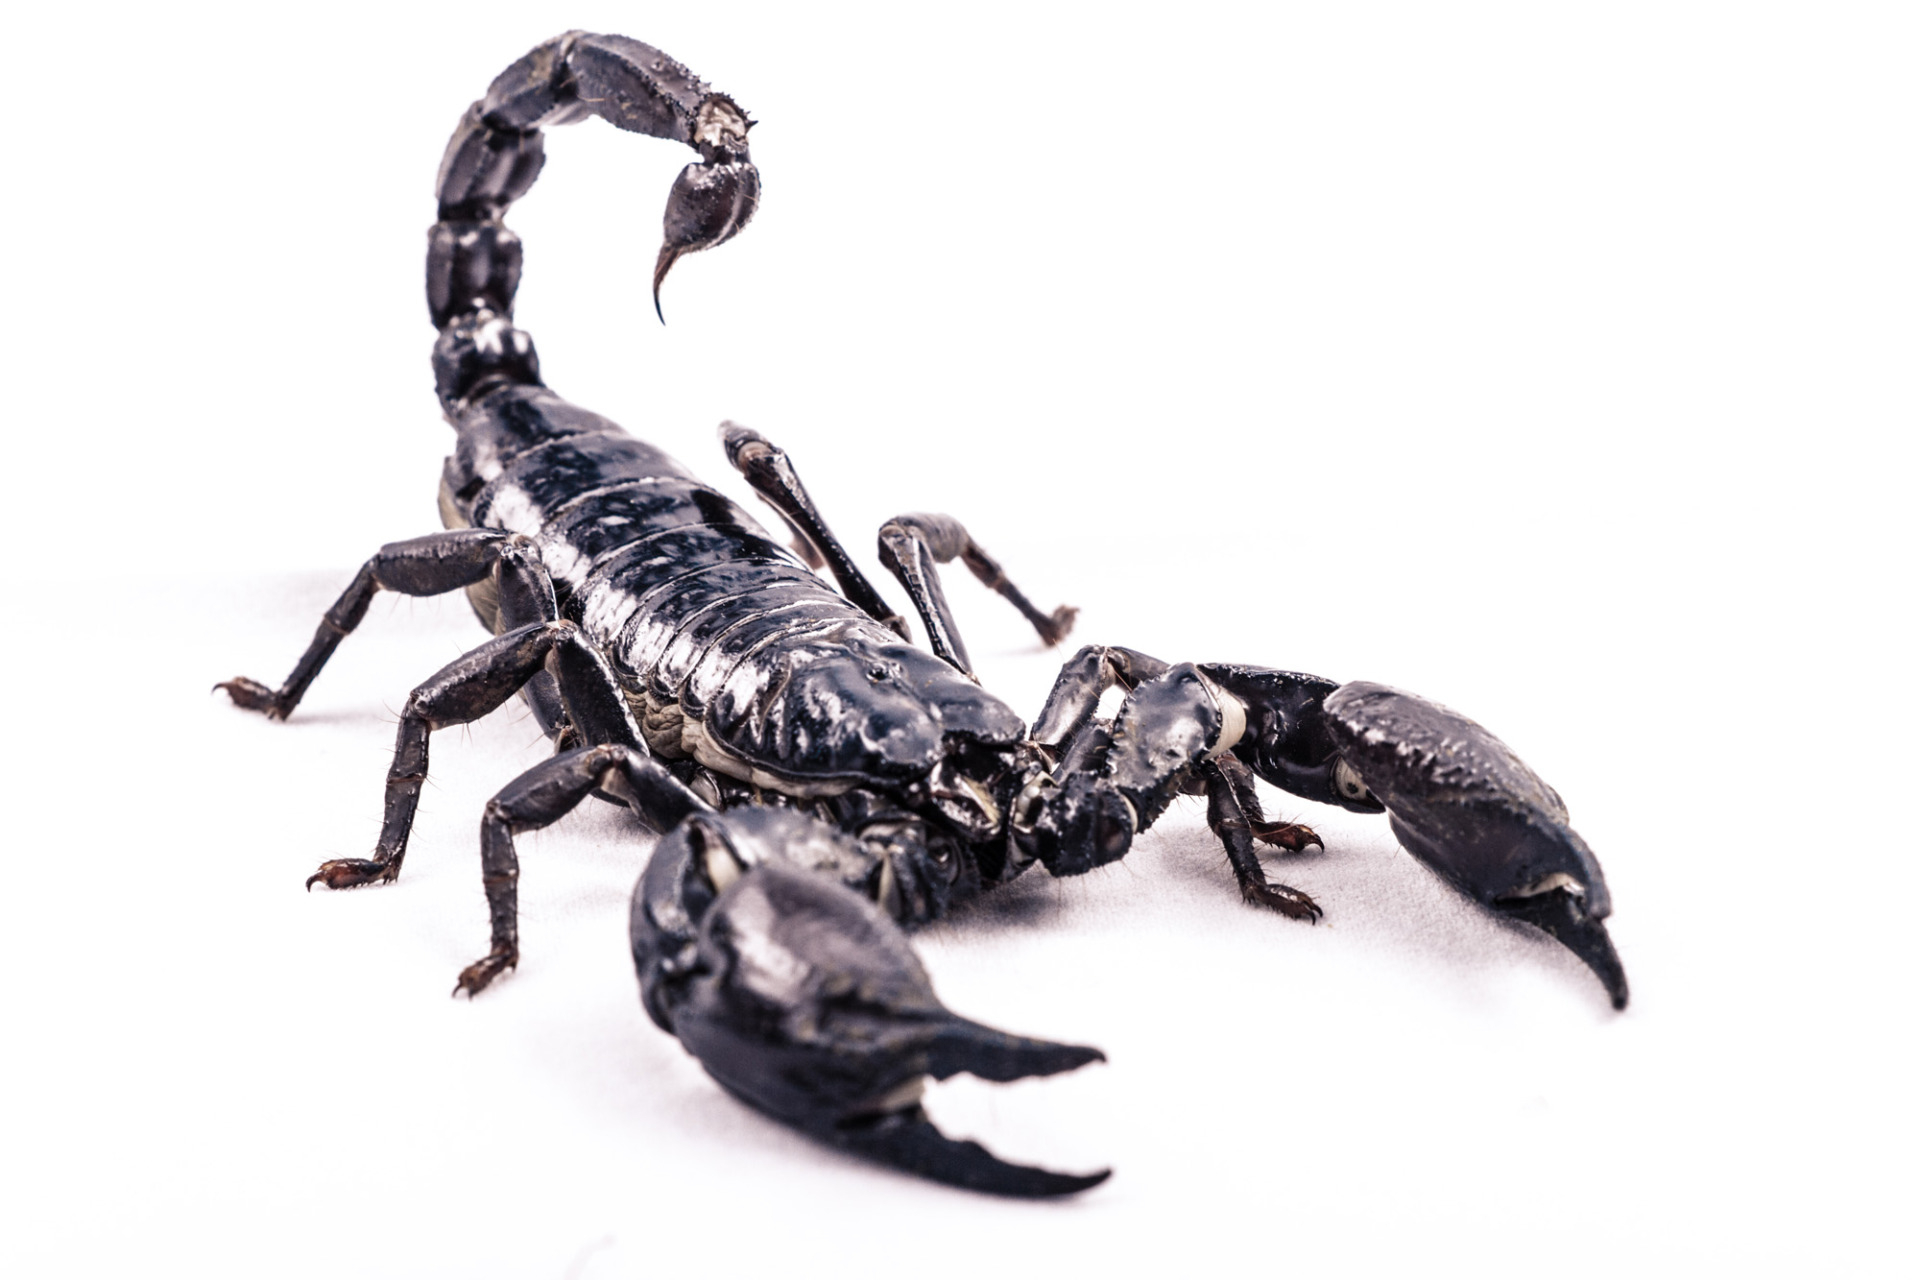
\includegraphics{figures/general/scorpion.jpg}}
    \else
    \fi
}

%---------------------------------------------------
% Equation helpers
\newcommand{\myvec}[1]{\ensuremath{\begin{pmatrix}#1\end{pmatrix}}}

\newcommand{\hl}[1]{{\color{red}#1}}


\newcommand\tenPlots[9]{%
    \def\tempa{#1}%
    \def\tempb{#2}%
    \def\tempc{#3}%
    \def\tempd{#4}%
    \def\tempe{#5}%
    \def\tempf{#6}%
    \def\tempg{#7}%
    \def\temph{#8}%
    \def\tempi{#9}%
    \tenPlotsContinued
}
\newcommand\tenPlotsContinued[3]{%
    %\newcommand{\tenPlots}[12]{
    \captionsetup[subfloat]{captionskip=5pt} % space between subfloat caption and image
    \begin{figure}[ht]
        \centering
        \subfloat[]{
            \includegraphics[width=0.32\textwidth]{\tempc} \hfill
            \label{\tempb-1}
        }
        \subfloat[]{
            \includegraphics[width=0.32\textwidth]{\tempd} \hfill
            \label{\tempb-2}
        }
        \subfloat[]{
            \includegraphics[width=0.32\textwidth]{\tempd} \hfill
            \label{\tempb-3}
        } \\
        \subfloat[]{
            \includegraphics[width=0.32\textwidth]{\tempf} \hfill
            \label{\tempb-4}
        }
        \subfloat[]{
            \includegraphics[width=0.32\textwidth]{\tempg} \hfill
            \label{\tempb-5}
        }
        \subfloat[]{
            \includegraphics[width=0.32\textwidth]{\temph} \hfill
            \label{\tempb-6}
        } \\
        \subfloat[]{
            \includegraphics[width=0.32\textwidth]{\tempi} \hfill
            \label{\tempb-7}
        }
        \subfloat[]{
            \includegraphics[width=0.32\textwidth]{#1} \hfill
            \label{\tempb-8}
        }
        \subfloat[]{
            \includegraphics[width=0.32\textwidth]{#2} \hfill
            \label{\tempb-9}
        } \\
        \subfloat[]{
            \includegraphics[width=0.32\textwidth]{#3} \hfill
            \label{\tempb-10}
        }
        {\caption{\tempa
                \label{\tempb} }}
    \end{figure}
    \captionsetup[subfloat]{captionskip=7pt} % space between subfloat caption and image
}

\newcommand\ninePlots[9]{%
    \def\tempa{#1}%
    \def\tempb{#2}%
    \def\tempc{#3}%
    \def\tempd{#4}%
    \def\tempe{#5}%
    \def\tempf{#6}%
    \def\tempg{#7}%
    \def\temph{#8}%
    \def\tempi{#9}%
    \ninePlotsContinued
}
\newcommand\ninePlotsContinued[2]{%
    %\newcommand{\tenPlots}[12]{
    \captionsetup[subfloat]{captionskip=5pt} % space between subfloat caption and image
    \begin{figure}[ht]
        \centering
        \subfloat[]{
            \includegraphics[width=0.32\textwidth]{\tempc} \hfill
            \label{\tempb-1}
        }
        \subfloat[]{
            \includegraphics[width=0.32\textwidth]{\tempd} \hfill
            \label{\tempb-2}
        }
        \subfloat[]{
            \includegraphics[width=0.32\textwidth]{\tempd} \hfill
            \label{\tempb-3}
        } \\
        \subfloat[]{
            \includegraphics[width=0.32\textwidth]{\tempf} \hfill
            \label{\tempb-4}
        }
        \subfloat[]{
            \includegraphics[width=0.32\textwidth]{\tempg} \hfill
            \label{\tempb-5}
        }
        \subfloat[]{
            \includegraphics[width=0.32\textwidth]{\temph} \hfill
            \label{\tempb-6}
        } \\
        \subfloat[]{
            \includegraphics[width=0.32\textwidth]{\tempi} \hfill
            \label{\tempb-7}
        }
        \subfloat[]{
            \includegraphics[width=0.32\textwidth]{#1} \hfill
            \label{\tempb-8}
        }
        \subfloat[]{
            \includegraphics[width=0.32\textwidth]{#2} \hfill
            \label{\tempb-9}
        } 
        {\caption{\tempa
                \label{\tempb} }}
    \end{figure}
    \captionsetup[subfloat]{captionskip=7pt} % space between subfloat caption and image
}

\newcommand{\fivePlots}[7]{
    \captionsetup[subfloat]{captionskip=5pt} % space between subfloat caption and image
    \begin{figure}[ht]
        \centering
        \subfloat[]{
            \includegraphics[width=0.32\textwidth]{#3} \hfill
            \label{#2-1}
        }
        \subfloat[]{
            \includegraphics[width=0.32\textwidth]{#4}
            \label{#2-2}
        }
        \subfloat[]{
            \includegraphics[width=0.32\textwidth]{#5} \hfill
            \label{#2-3}
        } \\
        \subfloat[]{
            \includegraphics[width=0.32\textwidth]{#6} \hfill
            \label{#2-4}
        }
        \subfloat[]{
            \includegraphics[width=0.32\textwidth]{#7} \hfill
            \label{#2-5}
        }
        {\caption{#1
                \label{#2} }}
    \end{figure}
    \captionsetup[subfloat]{captionskip=7pt} % space between subfloat caption and image
}

\newcommand{\sixPlots}[8]{
    \captionsetup[subfloat]{captionskip=5pt} % space between subfloat caption and image
    \begin{figure}[!ht]
        \centering
        \subfloat[]{
            \includegraphics[width=0.32\textwidth]{#3} \hfill
            \label{#2-1}
        }
        \subfloat[]{
            \includegraphics[width=0.32\textwidth]{#4} \hfill
            \label{#2-2}
        }
        \subfloat[]{
            \includegraphics[width=0.32\textwidth]{#5} \hfill
            \label{#2-3}
        } \\
        \subfloat[]{
            \includegraphics[width=0.32\textwidth]{#6} \hfill
            \label{#2-4}
        }
        \subfloat[]{
            \includegraphics[width=0.32\textwidth]{#7} \hfill
            \label{#2-5}
        }
        \subfloat[]{
            \includegraphics[width=0.32\textwidth]{#8} \hfill
            \label{#2-5}
        }
        {\caption{#1
                \label{#2} }}
    \end{figure}

    \captionsetup[subfloat]{captionskip=7pt} % space between subfloat caption and image
}
